\chapter{Condições de Contorno - Duto}\label{parte_1}

\begin{figure}[h!]
    \centering
    \hspace{-1.5cm}
    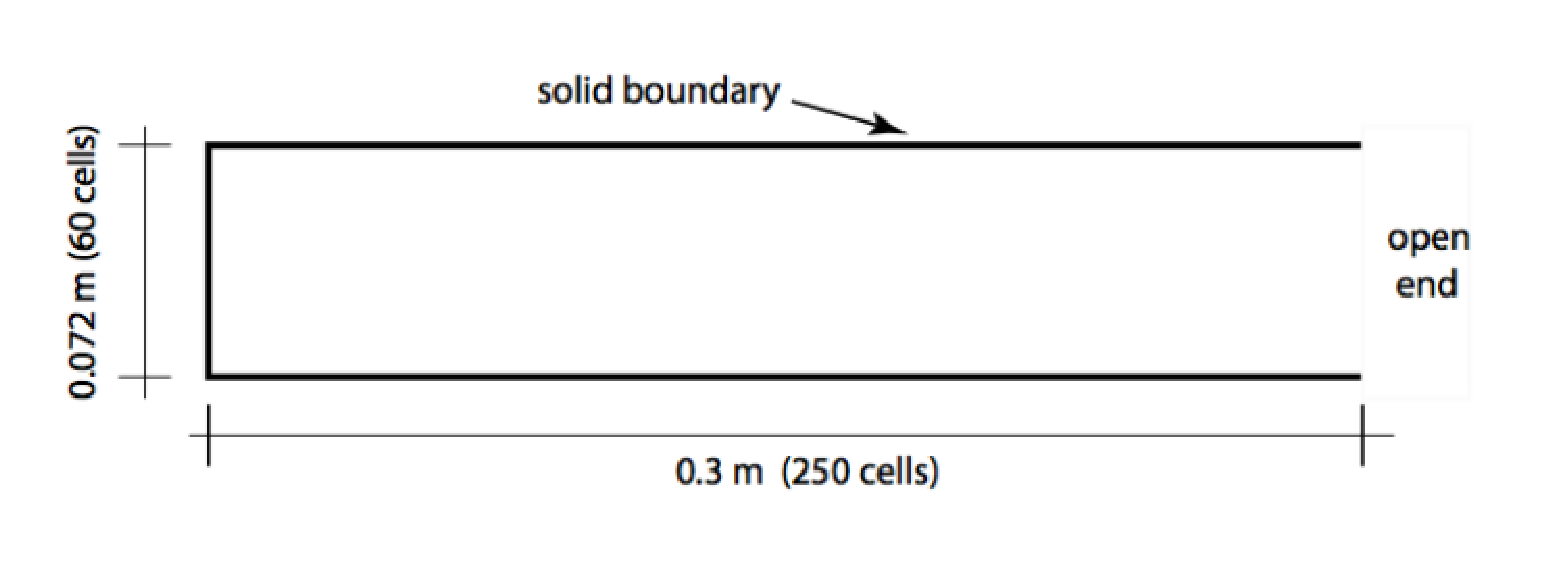
\includegraphics[width=0.8\textwidth]{figuras/duto.eps}
    \caption{Ilustração do duto abordado com a parede a direita aberta.}
\end{figure}

\section{Tubo Fechado-Fechado}
Nesse primeiro caso de simulação haverá um pulso de densidades em forma de uma linha de células de lattice na extremidade esquerda do tubo. Esse pulso irá se propagar até encontrar a condição fechada (barreira) ao final do duto. Ao encontrar essa condição a frente de onda de pressão é refletida com fase positiva. E assim a onda fará 8 vezes o caminho de ida e volta desse percurso. 

\subsection{Códigos}
\lstinputlisting{code_matlab/code_refactored/closed-closed/main_lbgk.m}
\lstinputlisting{code_matlab/code_refactored/closed-closed/build_lattice_D2Q9.m}
\lstinputlisting{code_matlab/code_refactored/closed-closed/set_initial_disturbances.m}
\lstinputlisting{code_matlab/code_refactored/closed-closed/calculate_velocities.m}
\lstinputlisting{code_matlab/code_refactored/closed-closed/collide_lattice.m}
\lstinputlisting{code_matlab/code_refactored/closed-closed/set_conditions_wall.m}
\lstinputlisting{code_matlab/code_refactored/closed-closed/stream_lattice.m}

\subsection{Imagens da Simulação}
\begin{figure}[h!]
    \centering
 	\hspace{-1.5cm}
    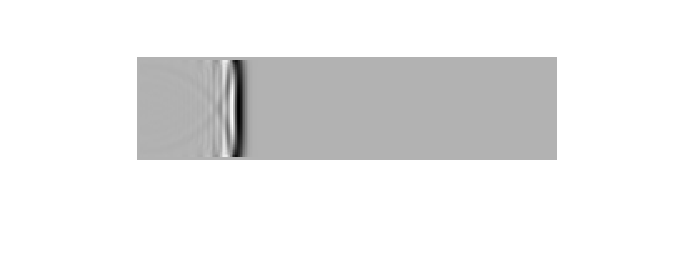
\includegraphics[width=0.8\textwidth]{code_matlab/code_refactored/closed-anechoic/normal.eps}
    \caption{Imagem da frente de onda indo em direção a parede.}
    \label{fig1}
\end{figure}
\begin{figure}[h!]
    \centering
 	\hspace{-1.5cm}
    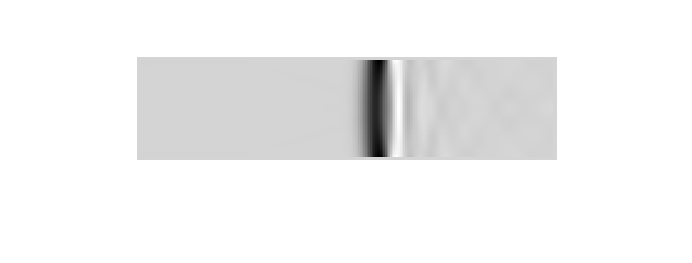
\includegraphics[width=0.8\textwidth]{code_matlab/code_refactored/closed-closed/print_c_c.eps}
    \caption{Imagem da frente de onda voltando depois da colisão com a parede do tubo fechado.}
    \label{fig2}
\end{figure}

\newpage
\subsection{Gráficos de Impedância}
\begin{figure}[h!]
    \centering
 	\hspace{-2.5cm}
    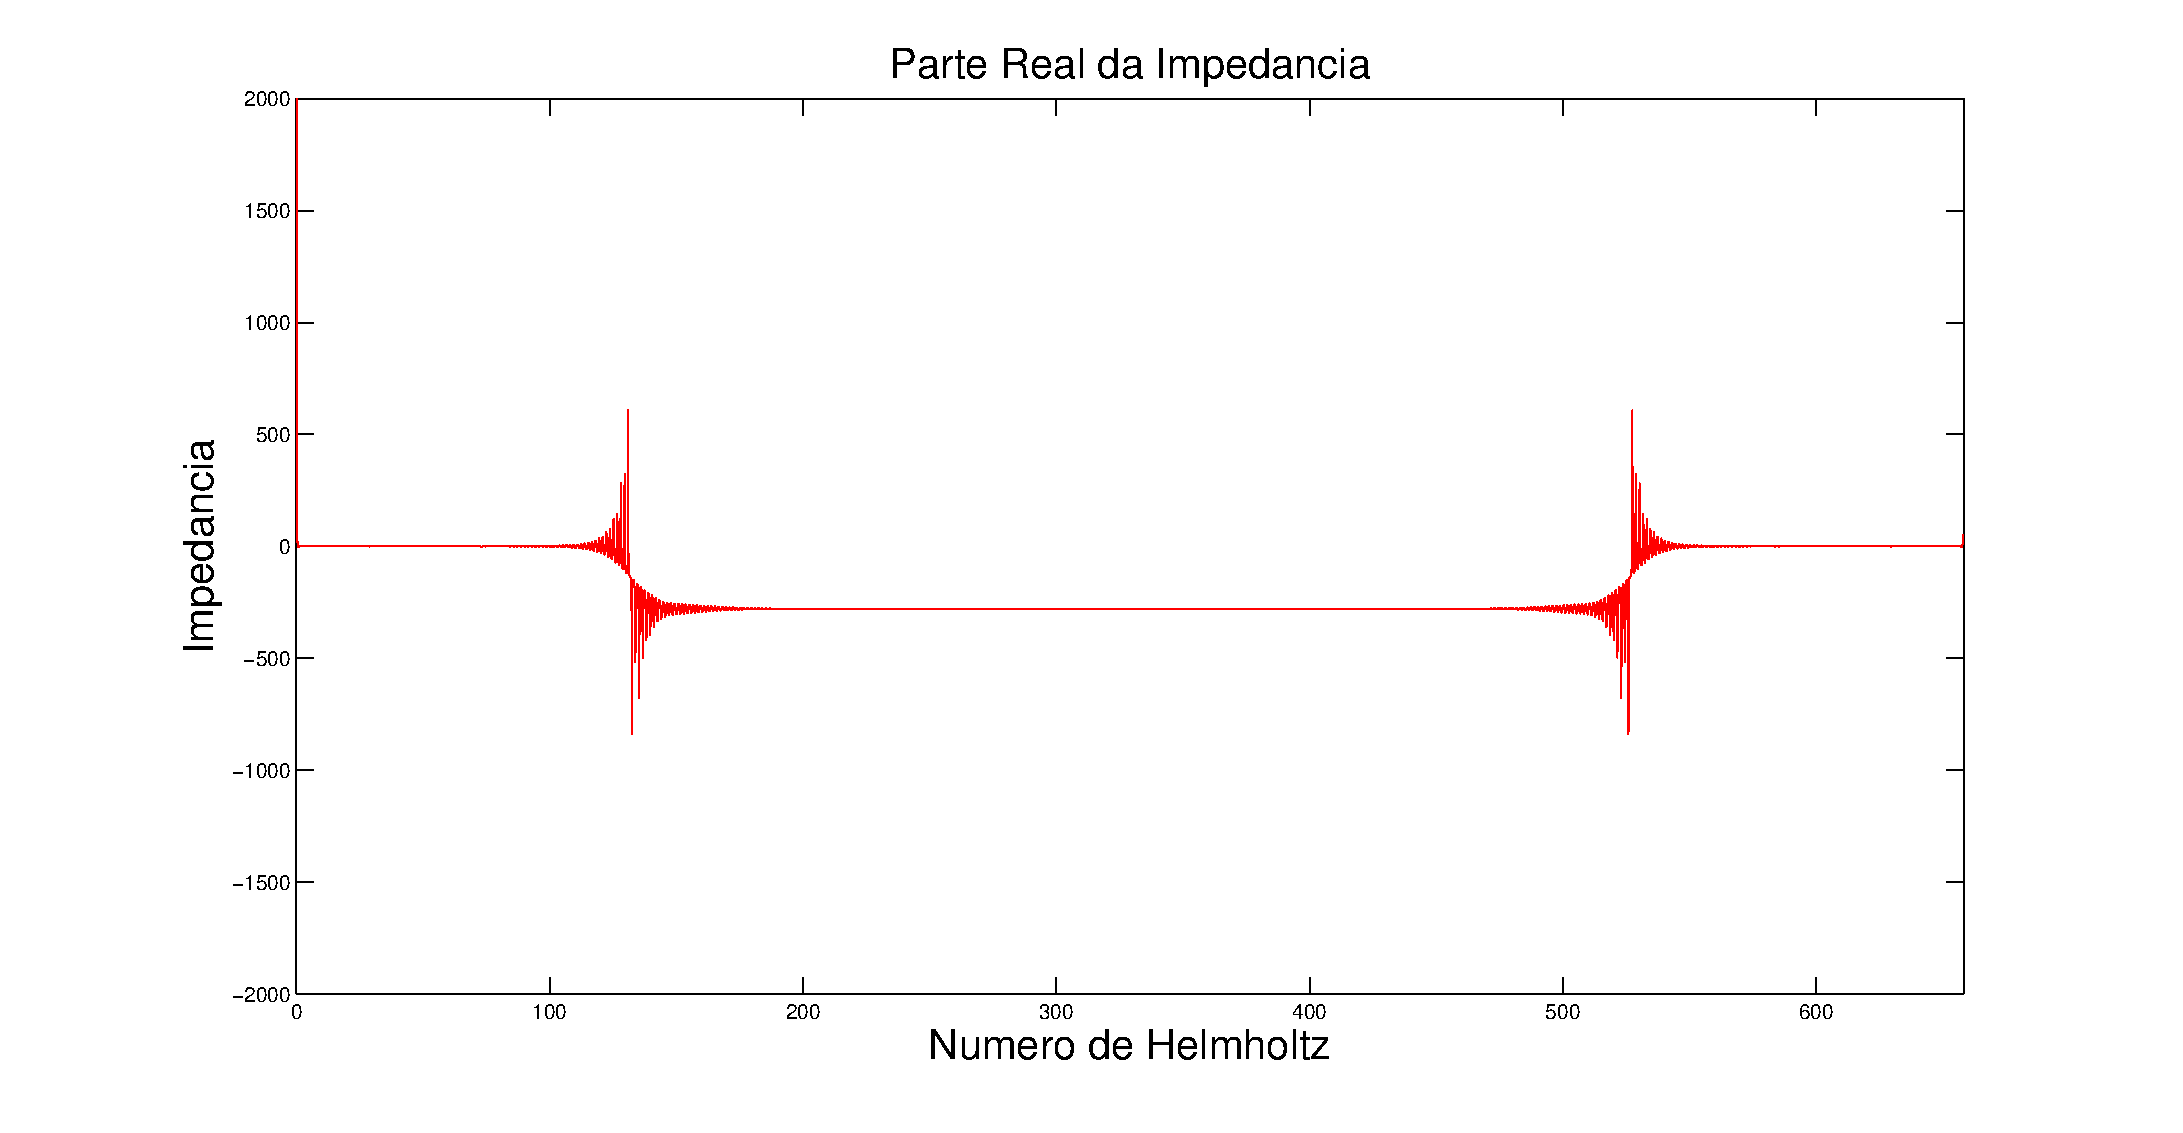
\includegraphics[width=1\textwidth]{code_matlab/code_refactored/closed-closed/parte_real_ativa.eps}
    \caption{Gráfico da parte real da impedância, ou seja, parte ativa de energia que não permanece no sistema.}
    \label{fig3}
\end{figure}
\begin{figure}[h!]
    \centering
 	\hspace{-2.5cm}
    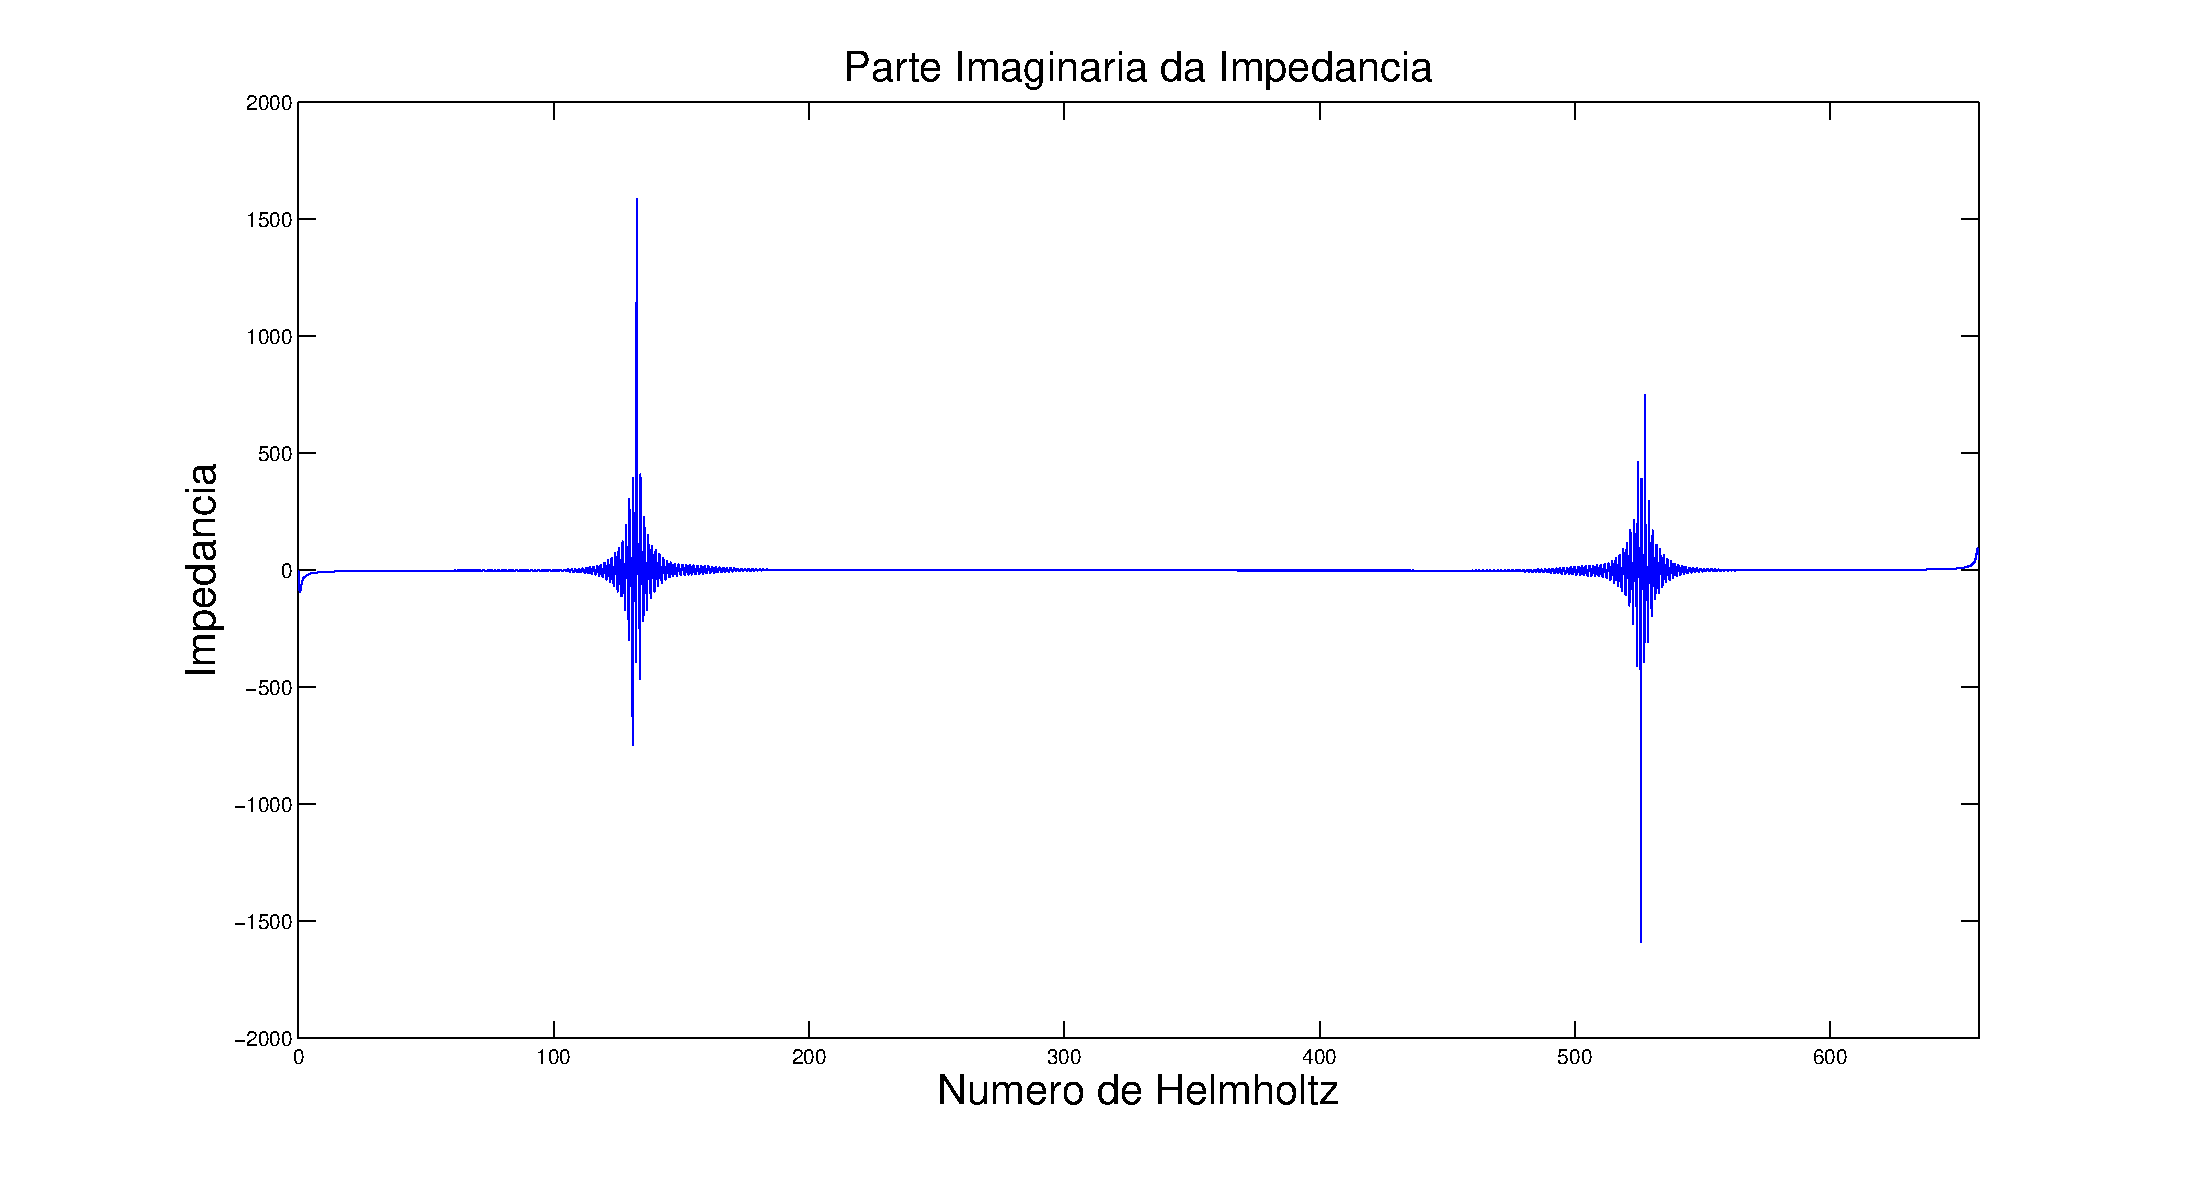
\includegraphics[width=1\textwidth]{code_matlab/code_refactored/closed-closed/parte_imaginaria_reativa.eps}
    \caption{Gráfico da parte imaginária da impedância, ou seja, parte reativa de energia que permanece no sistema.}
    \label{fig4}
\end{figure}

\subsection{Análise}

Em vista do que foi mostrado nas figuras \ref{fig1} e \ref{fig2}, de fato a onda colidiu com a parede, voltou com fase positiva e com bastante energia conservada. Também há de se comentar que o gráfico de maior energia foi o da figura \ref{fig4}. Esse fato confirma a hipótese de que, num duto de paredes fechadas, há pouquíssima energia (bem próxima de zero) se dissipando ou indo para fora do sistema (representado no gráfico da figura \ref{fig3}) e bastante energia contida dentro do tubo representado em \ref{fig4}. Também é perceptível que a parte real da impedância (ativa) decresce se aproximando de zero e a parte imaginária (reativa) cresce.
    
\newpage
\section{Tubo Fechado-Aberto}
Nesse segundo caso de simulação haverá um pulso de densidades em forma de uma linha de células de lattice na extremidade esquerda do tubo. Esse pulso irá se propagar até encontrar a condição aberta (sem nenhuma barreira ou condição de contorno) ao final do duto. Ao encontrar essa condição a frente de onda de pressão é refletida com fase negativa. E assim a onda fará 8 vezes o caminho de ida e volta desse percurso.

\subsection{Códigos}
\lstinputlisting{code_matlab/code_refactored/closed-opened/main_lbgk.m}


\subsection{Imagens da Simulação}
\begin{figure}[h!]
    \centering
 	\hspace{-1.5cm}
    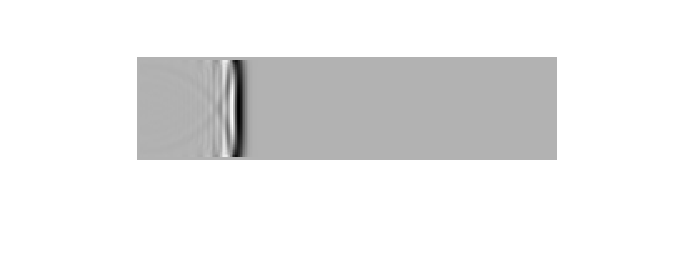
\includegraphics[width=1\textwidth]{code_matlab/code_refactored/closed-anechoic/normal.eps}
    \caption{Imagem da frente de onda indo em direção a parede.}
    \label{fig6}
\end{figure}
\begin{figure}[h!]
    \centering
 	\hspace{-1.5cm}
    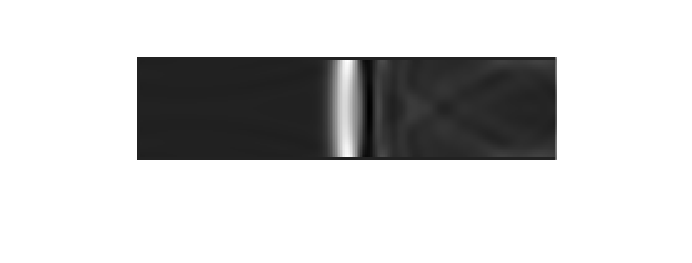
\includegraphics[width=1\textwidth]{code_matlab/code_refactored/closed-opened/print_c_o.eps}
    \caption{Imagem da frente de onda voltando depois da colisão com a parede do tubo aberto.}
    \label{fig7}
\end{figure}

\newpage
\subsection{Gráficos de Impedância}
\begin{figure}[h!]
    \centering
 	\hspace{-1.5cm}
    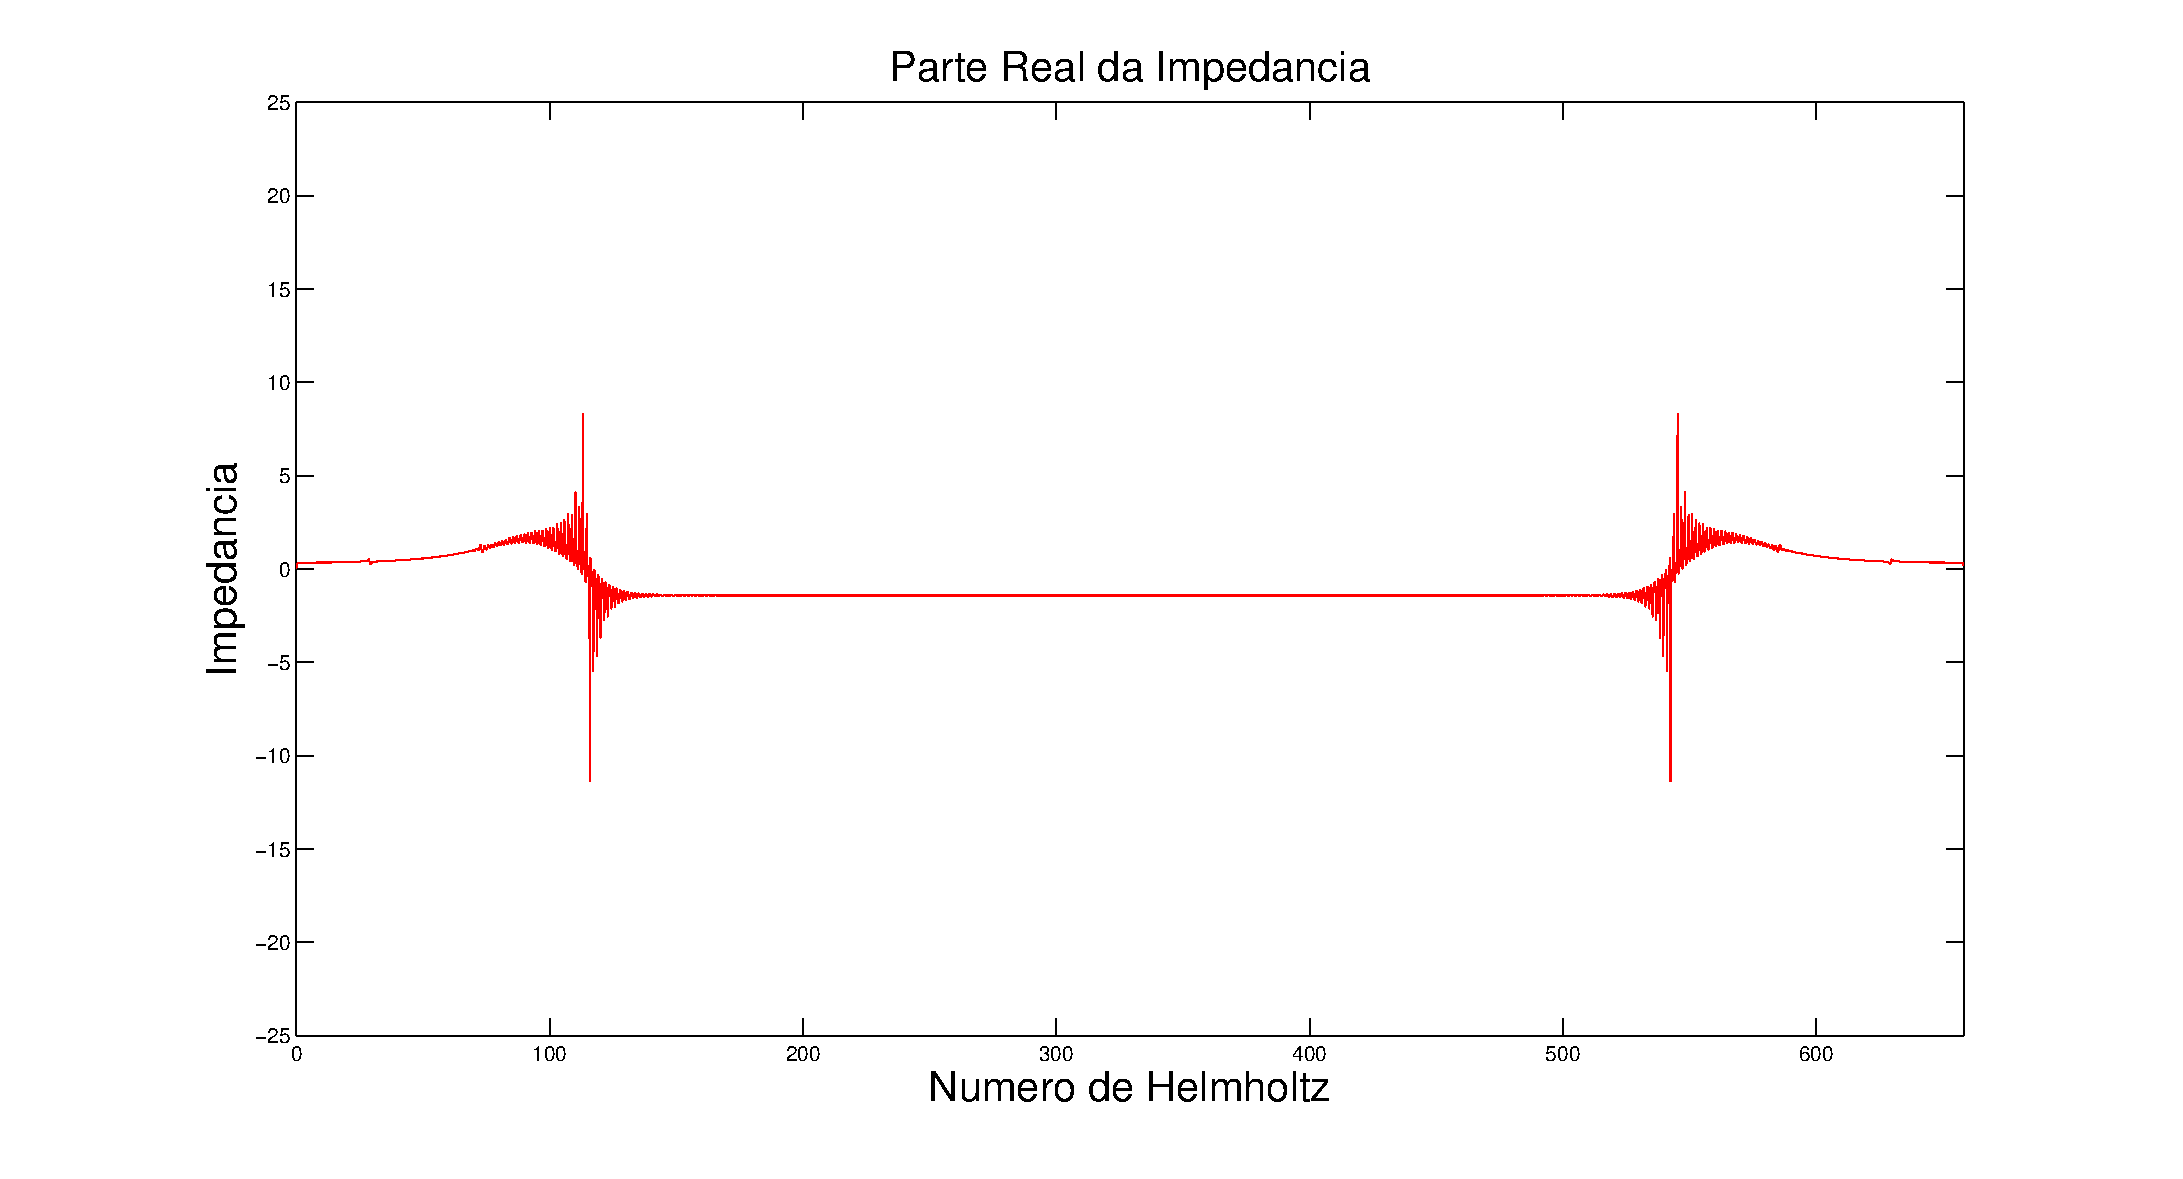
\includegraphics[width=1\textwidth]{code_matlab/code_refactored/closed-opened/parte_real_ativa.eps}
    \caption{Gráfico da parte real da impedância, ou seja, parte ativa de energia que não permanece no sistema.}
    \label{fig8}
\end{figure}
\begin{figure}[h!]
    \centering
 	\hspace{-1.5cm}
    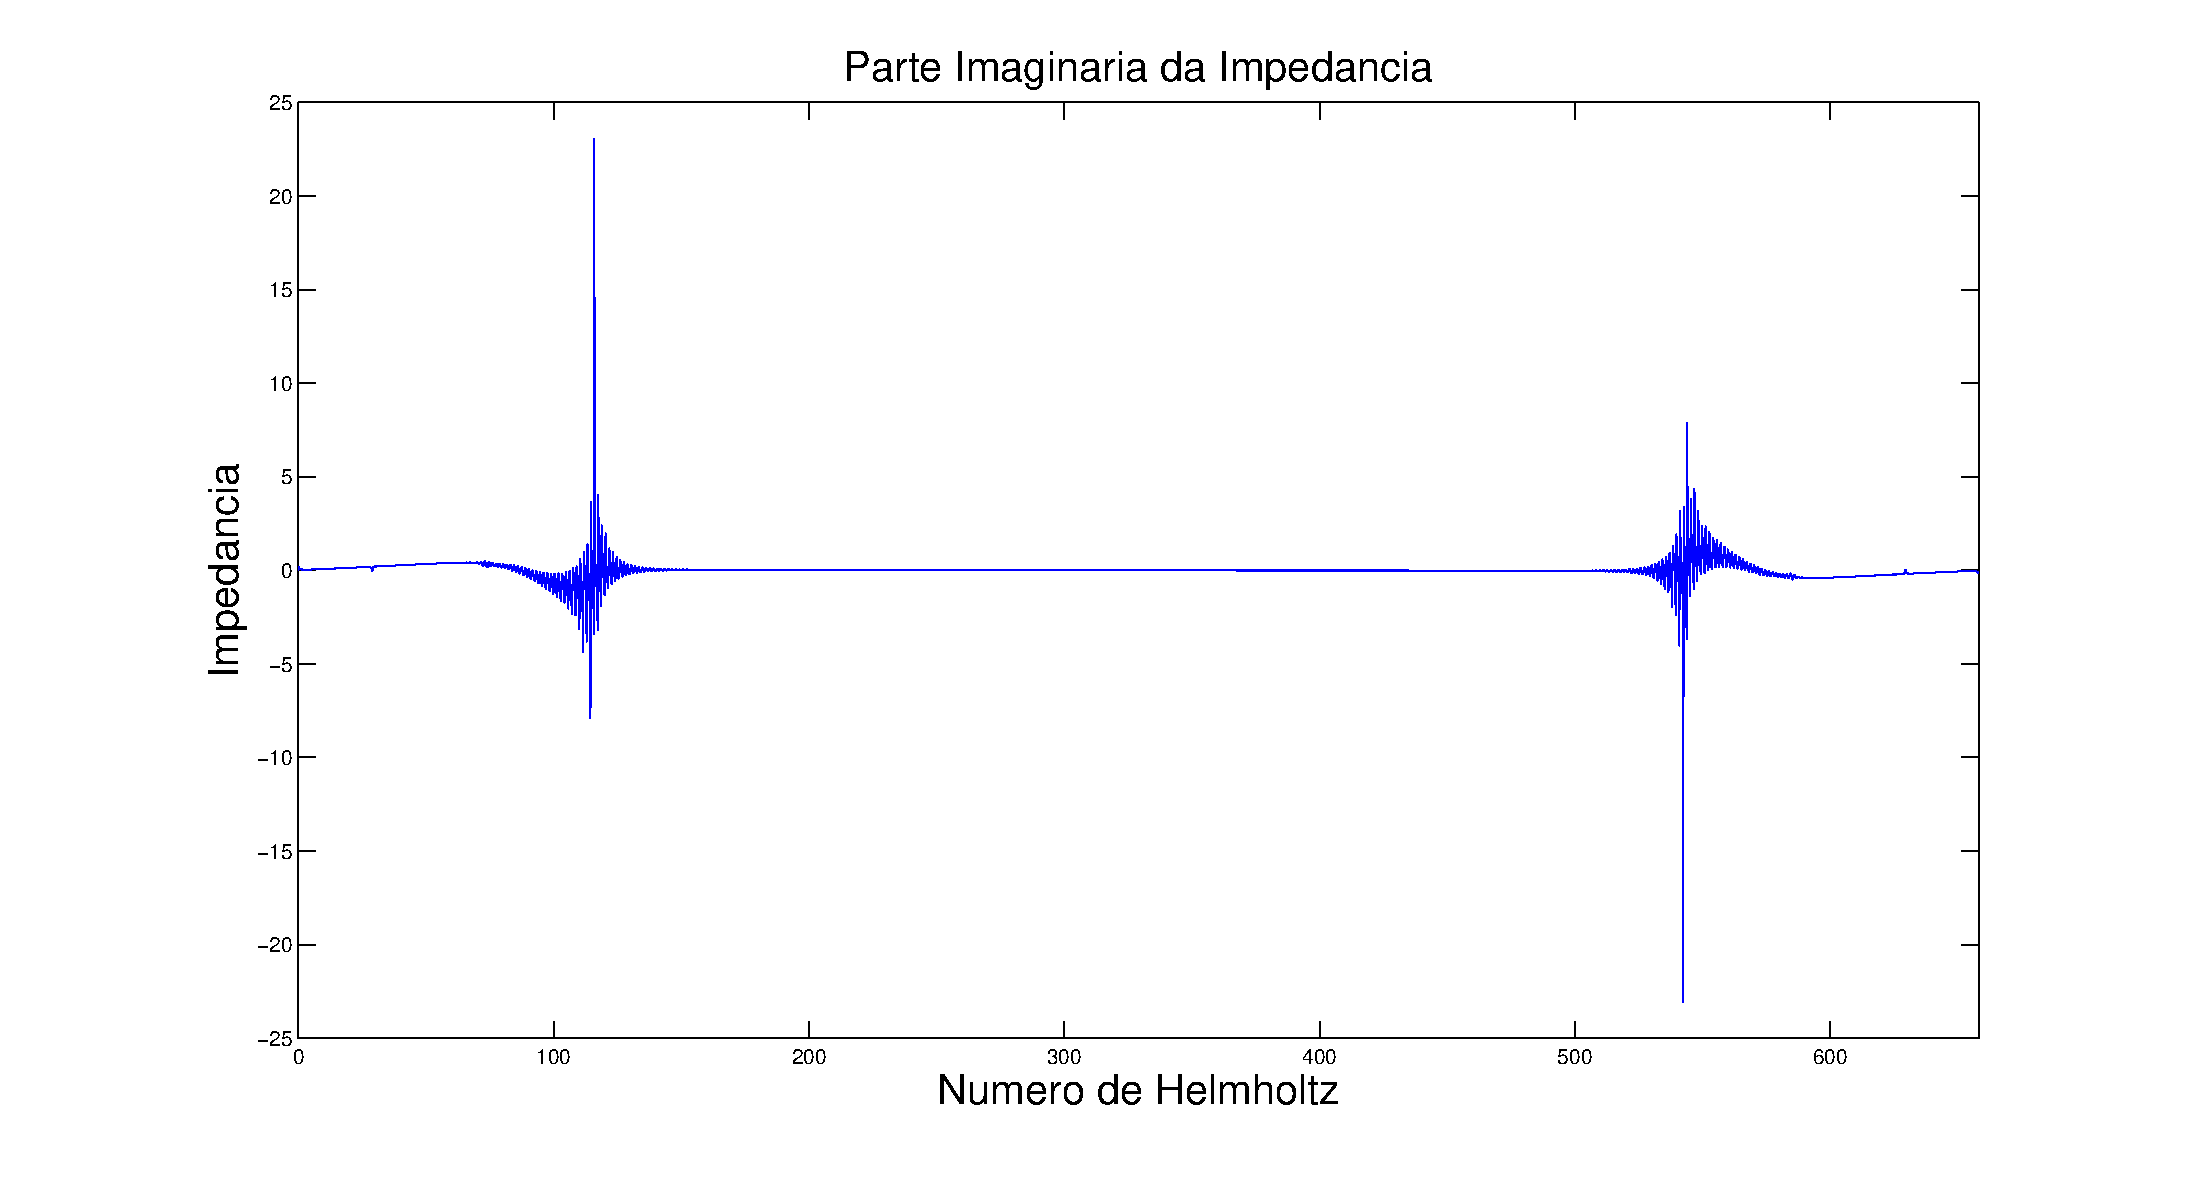
\includegraphics[width=1\textwidth]{code_matlab/code_refactored/closed-opened/parte_imaginaria_reativa.eps}
    \caption{Gráfico da parte imaginária da impedância, ou seja, parte reativa de energia que permanece no sistema.}
    \label{fig9}
\end{figure}

\subsection{Análise}

Em vista do que foi mostrado nas figuras \ref{fig6} e \ref{fig7}, de fato a onda colidiu com a parede e voltou com fase negativa, através de uma reflexão que não é de natureza propriamente física. Também há de se comentar que o gráfico de maior energia foi o da figura \ref{fig9}. Esse fato confirma a hipótese de que, devido as reflexões não físicas com a camada livre do duto, há pouquíssima energia se dissipando ou indo para fora do sistema (representado no gráfico da figura \ref{fig9}) e bastante energia se contida dentro do tubo representado em \ref{fig8}, porém a quantidade de energia ativa é maior do que é mostrado no mesmo caso para um duto fechado nas duas extremidades abordado anteriormente (figura \ref{fig3}).

\newpage
\section{Tubo Fechado-Aberto com tratamento ABC}

Nesse terceiro caso de simulação haverá um pulso de densidades em forma de uma linha de células de lattice na extremidade esquerda do tubo. Esse pulso irá se propagar até encontrar a condição aberta de tratamento anecóico (condição de contorno ABC) ao final do duto. Ao encontrar essa condição a frente de onda de pressão é absorvida.

\subsection{Códigos}
\lstinputlisting{code_matlab/code_refactored/closed-anechoic/main_lbgk.m}
\lstinputlisting{code_matlab/code_refactored/closed-anechoic/collide_lattice.m}

\subsection{Imagens da Simulação}
\begin{figure}[h!]
    \centering
 	\hspace{-1.5cm}
    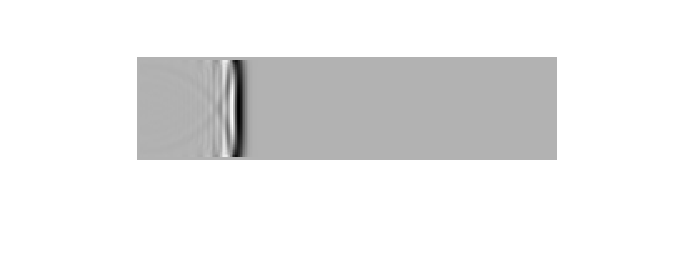
\includegraphics[width=0.9\textwidth]{code_matlab/code_refactored/closed-anechoic/normal.eps}
    \caption{Imagem da frente de onda indo em direção a parede.}
    \label{fig10}
\end{figure}
\begin{figure}[h!]
    \centering
 	\hspace{-1.5cm}
    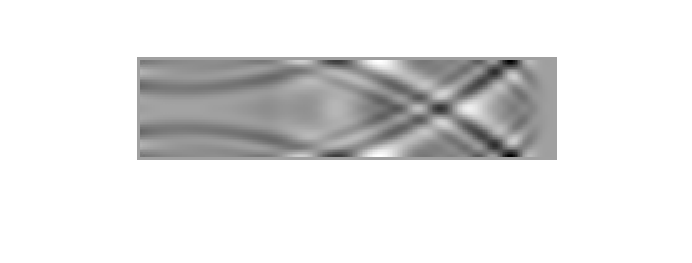
\includegraphics[width=0.9\textwidth]{code_matlab/code_refactored/closed-anechoic/print_c_a.eps}
    \caption{Imagem da frente de onda voltando depois da colisão com condição anecóica ao final.}
    \label{fig11}
\end{figure}

\newpage
\subsection{Gráficos de Impedância}
\begin{figure}[h!]
    \centering
 	\hspace{-1.5cm}
    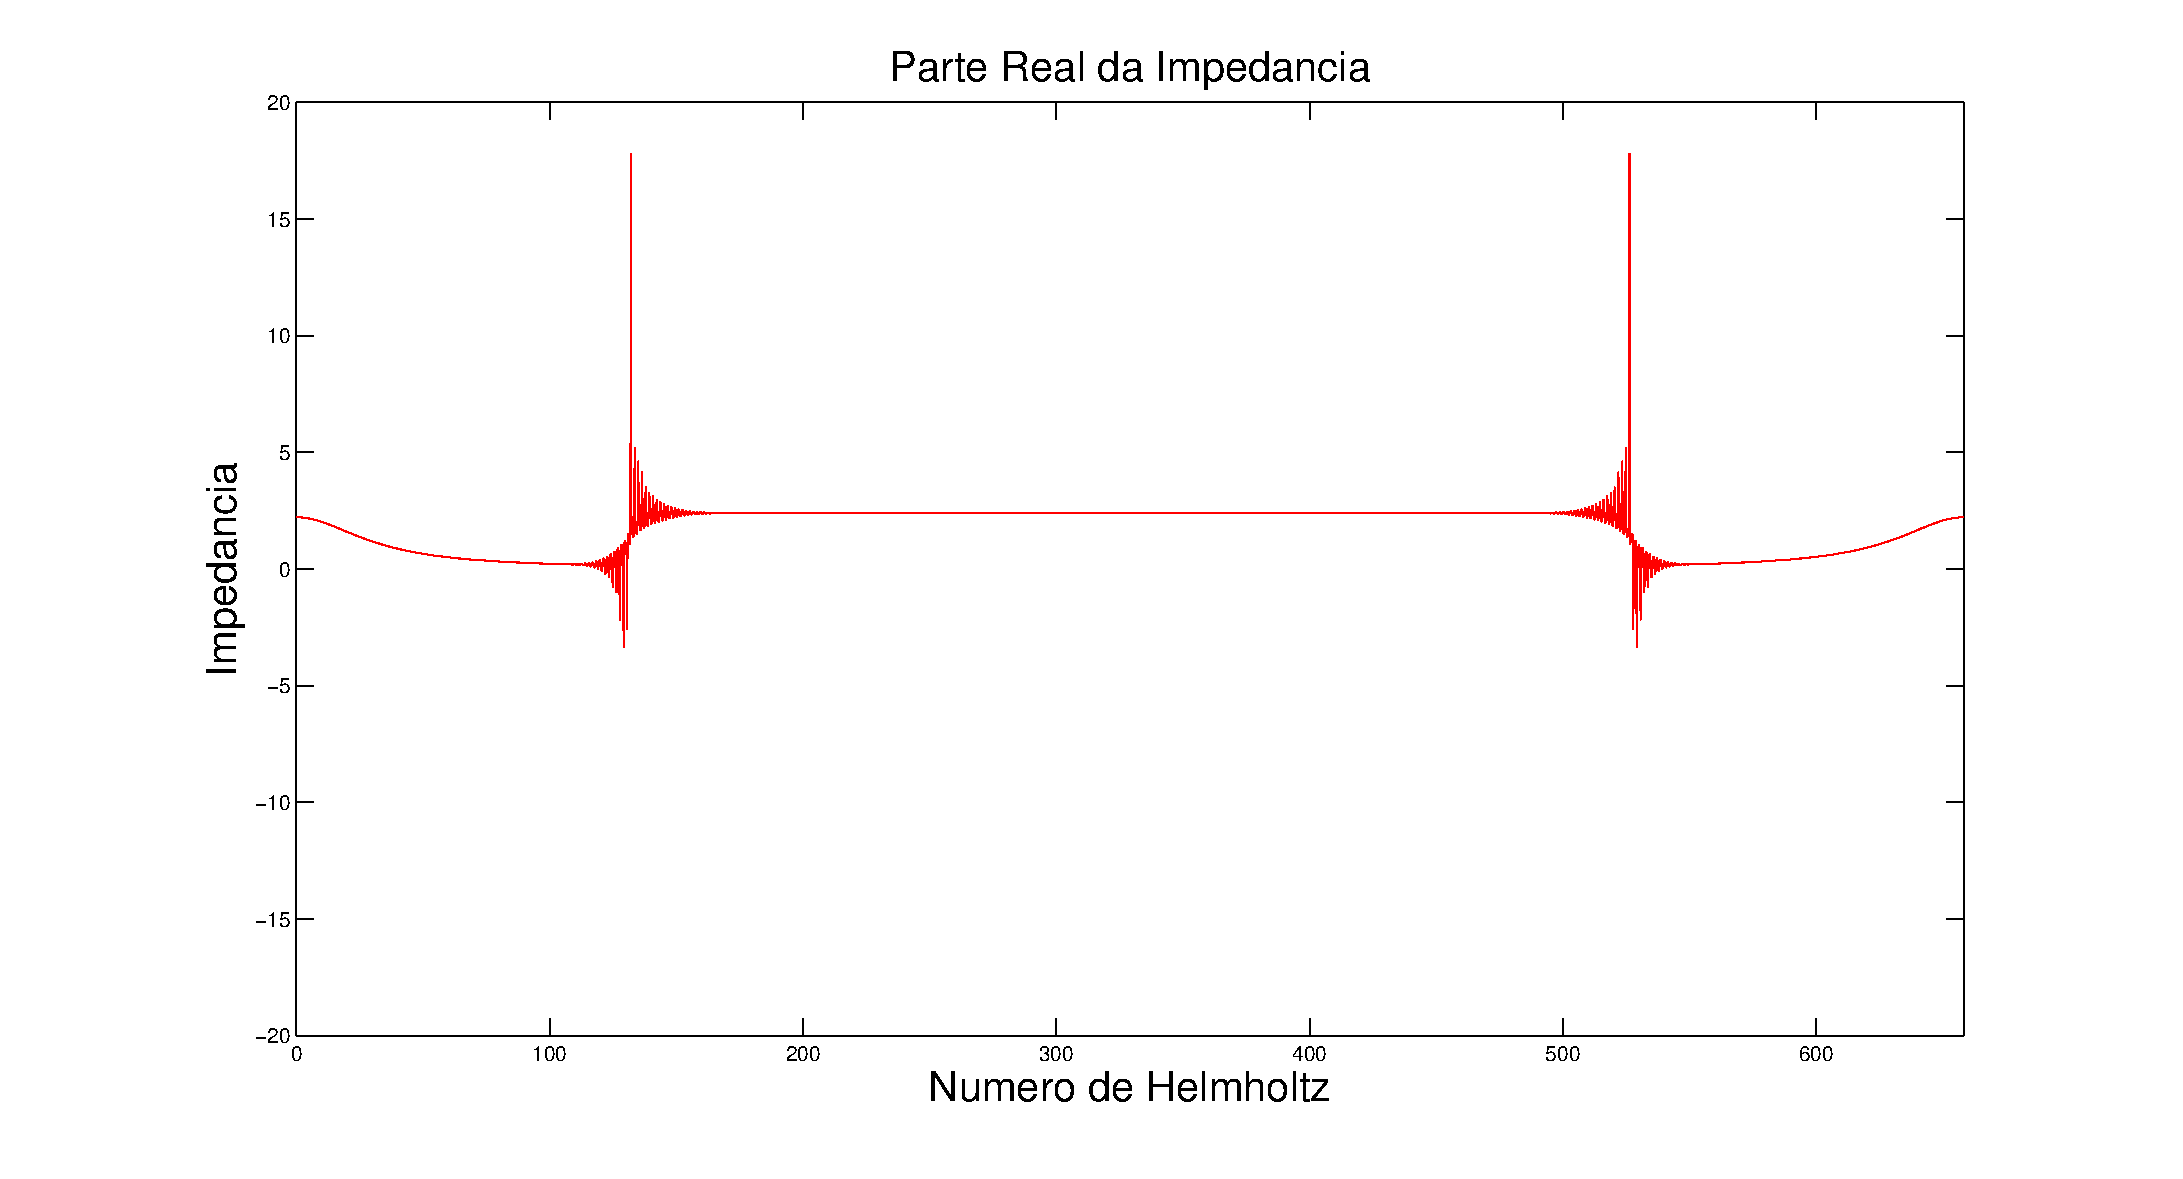
\includegraphics[width=1\textwidth]{code_matlab/code_refactored/closed-anechoic/parte_real_ativa.eps}
    \caption{Gráfico da parte real da impedância, ou seja, parte ativa de energia que não permanece no sistema.}
    \label{fig12}
\end{figure}
\begin{figure}[h!]
    \centering
 	\hspace{-1.5cm}
    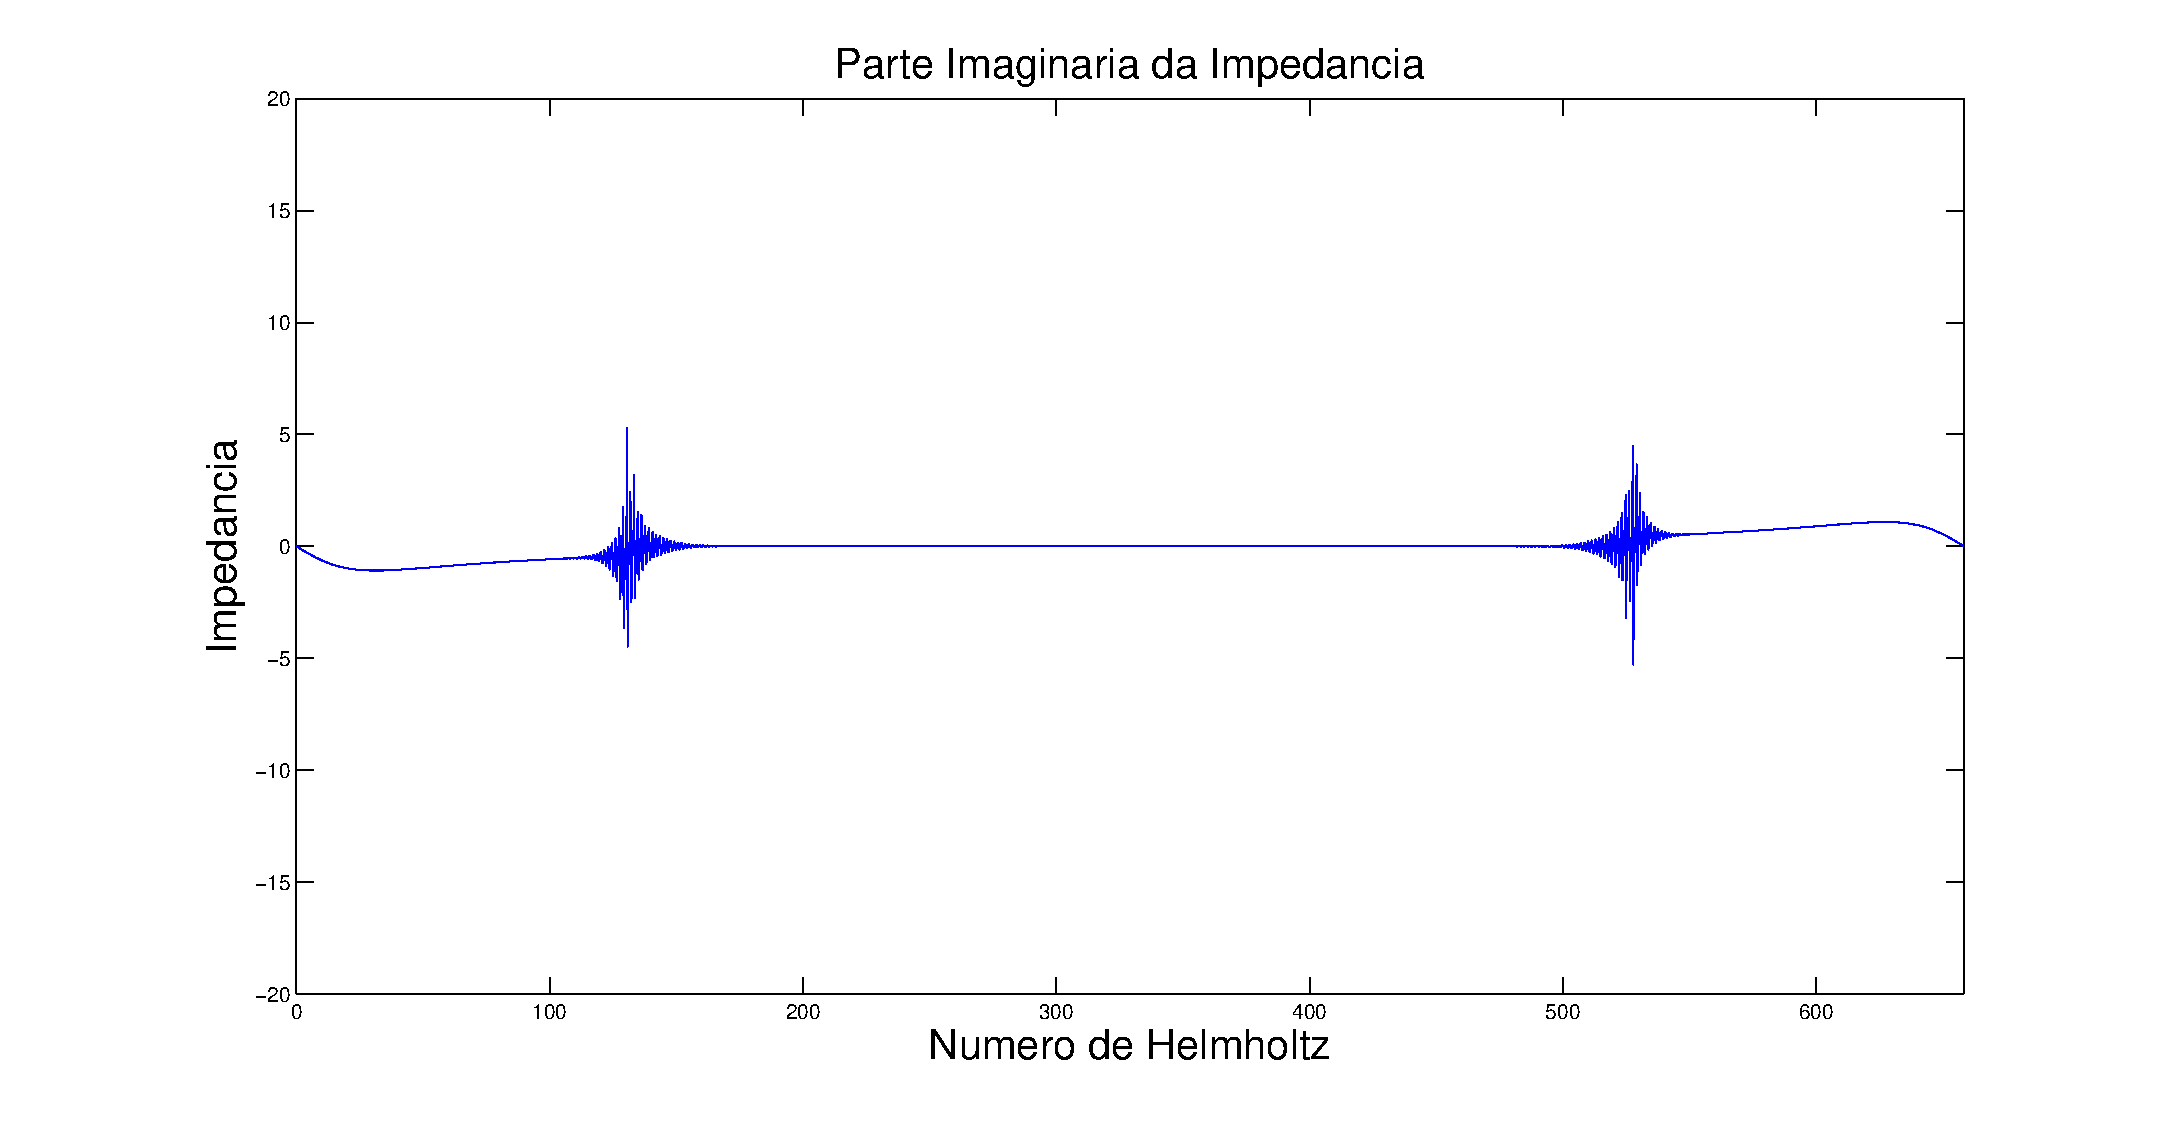
\includegraphics[width=1\textwidth]{code_matlab/code_refactored/closed-anechoic/parte_imaginaria_reativa.eps}
    \caption{Gráfico da parte imaginária da impedância, ou seja, parte reativa de energia que permanece no sistema.}
    \label{fig13}
\end{figure}

\section{Análise}
Em vista do que foi mostrado nas figuras \ref{fig10} e \ref{fig11}, de fato a onda colidiu com a condição anecóica ABC e foi absorvida. Também há de se comentar que o gráfico de maior energia foi o da figura \ref{fig12}. Esse fato confirma a hipótese de que, devido a condição anecóica no final do duto, há bastante energia se dissipando ou indo para fora do sistema (representado no gráfico da figura \ref{fig12}) e pouca energia contida dentro do tubo representado em \ref{fig11}.

\chapter{Filtro Acústico - Muffler}\label{parte_1}

\begin{figure}[h!]
    \centering
    \hspace{-2.5cm}
    \includegraphics[width=1.2\textwidth]{/home/gepeto/jose_pedro/muffler/print_muffler_desenho.eps}
    \caption{Ilustração esquemática do muffler.}
    \label{fig13}
\end{figure}

Nessa simulação foi implementado um muffler de acordo com o que é mostrado em \ref{fig13}. Além da estrutura de paredes e condições anecóicas nas extremidades, foi colocado uma perturbação $chirp$ na extremidade esquerda através de inserção de massa na implementação de contorno ABC. Essa perturbação $chirp$ vai de 0 até 16kHz em unidades físicas ao longo da metade do tempo de simulação, deixando outra metade para propagação das ondas e excitação das frequências de ressonâncias do tubo.

\section{Códigos}
\lstinputlisting{/home/gepeto/jose_pedro/muffler/main_lbgk.m}

\newpage
\section{Imagens da Simulação}
\begin{figure}[h!]
    \centering
    \hspace{-1.5cm}
    \includegraphics[width=0.7\textwidth]{/home/gepeto/jose_pedro/muffler/print_muffler_1.eps}
    \caption{Muffler sendo excitado ainda no começo antes da metade do tempo de simulação.}
    \label{fig14}
\end{figure}
\begin{figure}[h!]
    \centering
    \hspace{-1.5cm}
    \includegraphics[width=0.7\textwidth]{/home/gepeto/jose_pedro/muffler/print_muffler_2.eps}
    \caption{Muffler depois de excitado ressonando para a primeira frequência.}
    \label{fig15}
\end{figure}
\begin{figure}[h!]
    \centering
    \hspace{-1.5cm}
    \includegraphics[width=0.7\textwidth]{/home/gepeto/jose_pedro/muffler/print_muffler_3.eps}
    \caption{Muffler depois de excitado ressonando para a segunda frequência.}
    \label{fig16}
\end{figure}

\newpage
\section{Gráfico da Atenuação}
\begin{figure}[h!]
    \centering
    \hspace{-1.5cm}
    \includegraphics[width=1.2\textwidth]{/home/gepeto/jose_pedro/muffler/perda_transmissao.eps}
    \caption{Comparação da curva obtida com elementos finitos e com a curva da simulação.}
    \label{fig17}
\end{figure}

\section{Análise}
Em vista do que foi mostrado nas figuras \ref{fig14}, \ref{fig15} e \ref{fig16}, a excitação do tipo $chirp$ realmente estava mandando pulsos cada vez mais frequentes e rápidos para o muffler sem o estouro da $lattice$ por emissão de massa em excesso e também é observado que depois da metade do tempo de simulação, depois que o $chirp$ termina o processo de perturbação, dois modos de ressonância surgem com energia acumulada. Também há de se comentar que o gráfico \ref{fig17} de perda de transmissão realmente mostrou dois picos para os dois modos excitados vistos nas imagens da simulação, porém o mesmo divergiu significamente da curva de referência feita em elementos finitos. Visivelmente percebe que outros modos não foram excitados e que os modos excitados estão deslocados, no entanto, a curva segue uma tendência grosseira e sem muito ruído.
